% Version 4: Figures
\documentclass[11pt]{beamer}

%\usetheme{Marburg}
\usetheme{Madrid}
\setbeamertemplate{navigation symbols}{}

\usepackage{tikz}
\usetikzlibrary{arrows,shapes.geometric,shapes.symbols,scopes}
\colorlet{DarkRed}{red!70!black}
\colorlet{DarkBlue}{blue!70!black}
\colorlet{DarkGreen}{green!50!black}

\logo{
\includegraphics[height=0.5cm]{ssn-logo.jpg}}
\title{Presentation in \LaTeX}
\author[Milton]{R~S~Milton}
\institute[]{
  Department of Computer Science\\
  SSN College of Engineering
}

\date[]{18 February 2016}

\renewcommand{\emph}[1]{\textcolor{magenta}{#1}}

\begin{document}

\begin{frame}
  \titlepage
\end{frame}

\begin{frame}{Outline of the talk}
  \tableofcontents
\end{frame}


\section{Quick presentation}

\begin{frame}{Simple presentation}
  With LaTeX Beamer, we can make consistently looking
  presentation.
  \begin{itemize}
  \item Use \texttt{beamer} class.
  \item Choose a theme.
  \item Otherwise, usual \LaTeX.
  \end{itemize}
\end{frame}

\begin{frame}
  \frametitle{Simplicity}
  Use simple and direct words.
  \begin{block}{Herman Melville}
    A man of true science \ldots uses but few hard words, and
    those only when none other will answer his purpose; whereas
    the smatterer in science\ldots thinks, that by mouthing
    hard words, he proves that he understands hard things.
  \end{block}
  \begin{alertblock}{Herman Melville}
    A man of true science \ldots uses but few hard words, and
    those only when none other will answer his purpose.
  \end{alertblock}
  \begin{exampleblock}
    {Herman Melville}
    A man of true science \ldots uses but few hard words, and
    those only when none other will answer his purpose.
  \end{exampleblock}
\end{frame}

\begin{frame}
  \frametitle{Two columns}
  Use simple and direct words.
  \begin{columns}
    \begin{column}{.45\textwidth}
      \begin{block}{Herman Melville}
        A man of true science \ldots uses but few hard words,
        and those only when none other will answer his purpose;
        whereas the smatterer in science\ldots thinks, that by
        mouthing hard words, he proves that he understands hard
        things.
      \end{block}
    \end{column}
    \begin{column}{.45\textwidth}
      \begin{alertblock}{Herman Melville}
        A man of true science \ldots uses but few hard words,
        and those only when none other will answer his purpose;
        whereas the smatterer in science\ldots thinks, that by
        mouthing hard words, he proves that he understands hard
        things.
      \end{alertblock}
    \end{column}
  \end{columns}
\end{frame}

\begin{frame}
  \frametitle{Two column use}
  \begin{columns}
    \begin{column}{.4\textwidth}
    \begin{center}
      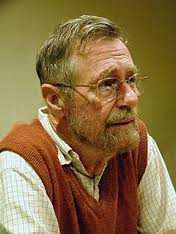
\includegraphics[scale=.5]{dijkstra.jpeg}
    \end{center}      
    \end{column}
    \begin{column}{.5\textwidth}
      \begin{exampleblock}{What is Computer Science?}
        Computer Science is no more about computers than
        astronomy is about telescopes or biology is about
        microscopes (E W Dijkstra).
      \end{exampleblock}
    \end{column}
  \end{columns}
\end{frame}


\begin{frame}
  \frametitle{Pause}
  \begin{block}{Herman Melville}
    A man of true science \ldots \pause uses but few hard
    words, \pause and those only when none other will answer
    his purpose; \pause whereas the smatterer in science\ldots
    \pause thinks, that by mouthing hard words, he proves that
    he understands hard things.
  \end{block}
\end{frame}

\begin{frame}
  \frametitle{On certain slides}
  \begin{block}{Herman Melville}
    \onslide<2-3>{It is better to fail in originality, than to
      succeed in imitation. }%
    \onslide<3>{\emph{He who has never failed somewhere, that
        man can not be great.} }%
    \onslide<1-3>{Failure is the true test of greatness.}
  \end{block}
\end{frame}


\begin{frame}
  \frametitle{Stepwise revelation}
  \begin{columns}
    \begin{column}{.5\textwidth}
      \begin{itemize}
      \item<1-> First step.
      \item<2-> Second step.
      \item<3-> Third step.
      \end{itemize}
    \end{column}
    \begin{column}{.5\textwidth}
      \begin{itemize}
      \item<1-> First step.
      \item<2-> Second step.
      \item<3-> Third step.
      \end{itemize}
    \end{column}
  \end{columns}
\end{frame}

\begin{frame}
  \frametitle{Stepwise revelation}
  \begin{minipage}{.45\linewidth}
    \begin{itemize}[<+->]
    \item First step.
    \item Second step.
    \item Third step.
    \end{itemize}
  \end{minipage}
  \begin{minipage}{.45\linewidth}
    \begin{itemize}[<+- | alert@+>]
    \item First step.
    \item Second step.
    \item Third step.
    \end{itemize}
  \end{minipage}
\end{frame}

\begin{frame}
  \frametitle{Stepwise revelation}
  \begin{tabular}{ll}
    \onslide<1->{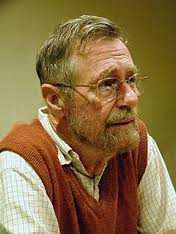
\includegraphics[width=2cm]{dijkstra.jpeg}} & \onslide<1->{E W Dijkstra}\\
    \onslide<2->{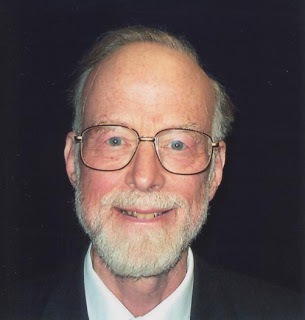
\includegraphics[width=2cm]{hoare.jpeg}} & \onslide<2->{C A R Hoare}\\
    \onslide<3->{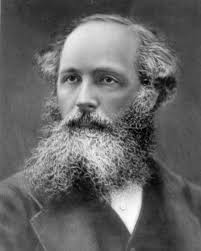
\includegraphics[width=2cm]{maxwell.jpeg}} & \onslide<3->{J C Maxwell}
  \end{tabular}
\end{frame}

\section{Figures}

\begin{frame}
  \frametitle{Figures}
  \begin{minipage}{.45\linewidth}
    \begin{center}
      % \documentclass{article}

% \usepackage{tikz}
% \usetikzlibrary{arrows,shapes.geometric,shapes.symbols,scopes}

% \colorlet{DarkRed}{red!70!black}
% \colorlet{DarkBlue}{blue!70!black}
% \colorlet{DarkGreen}{green!50!black}

% \begin{document}

% Define block styles
\tikzstyle{block} = [rectangle, draw, draw=DarkBlue, inner
color=DarkBlue!0!white, outer color=DarkBlue!15!white,
text width=10em, thick,text centered, minimum height=2em] %

%\tikzstyle{line} = [draw, -latex']%
\tikzstyle{oval} = [rectangle, draw, draw=DarkGreen, fill=green!10, text width=10em, thick, text centered, rounded corners, minimum height=2em] %
\tikzstyle{arrow} = [thick,draw=DarkGreen,->,>=stealth]

\begin{tikzpicture}[node distance = 1.7cm, auto]
  % Place nodes
  \node [oval](in) {IE Extractions};
  \node [block, below of=in] (pc) {Predicate Counting};
  \node [block, below of=pc] (dg) {Graph Construction};
  \node [block, below of=dg] (gr) {Ground Rules Generation};
  \node [oval, below of=gr] (for) {First Order Rules};
  
  % Draw edges
  \draw [arrow] (in) -- (pc);
  \draw [arrow] (pc) -- (dg);
  \draw [arrow] (dg) -- (gr);
  \draw [arrow] (gr) -- (for);
\end{tikzpicture}
%\end{document}

    \end{center}
  \end{minipage}
  \begin{minipage}{.45\linewidth}
    \begin{center}
      % /home/milton/csedept/talks/latex-2016/rule-learner2.jdr
% Created by FlowframTk version 0.8.2
% 18 Feb, 2016 1:21:11 PM
\iffalse
% This image may require the following commands in the preamble:
\usepackage{ifpdf}
\makeatletter
\newcommand*{\jdroutline}[3]{%
  \GenericWarning{}{text outline can't be implemented}#3%
}%
\ifpdf
 \let\jdrorgmod\mod
 \InputIfFileExists{pdf-trans}%
 {%
   \renewcommand*{\jdroutline}[3]{%
     {\def\mod{\expandtwonumexprafter \modulo}%
     \setbox\@tempboxa\hbox{##3}%
     \boxgs{##1}{}\copy\@tempboxa
     }%
   }%
 }{}
 \let\mod\jdrorgmod
\else
 \IfFileExists{pst-char.sty}%
 {%
   \usepackage{pst-char}
   \renewcommand*{\jdroutline}[3]{%
     \begin{pspicture}(0,0)
     \pscharpath[##2]{##3}
     \end{pspicture}
   }
 }{}
\fi
\makeatother
\usepackage{pgf}
\usepgflibrary{decorations.text}
% The normal size font is assumed to be 10pt
% End of preamble information
\fi
\begin{pgfpicture}
\pgfpathmoveto{\pgfpoint{4.5bp}{424.775591bp}}
\pgfpathlineto{\pgfpoint{86.671875bp}{590.775591bp}}
\pgfusepath{use as bounding box}
\begin{pgfscope}
\pgftransformcm{1.0}{-0.0}{0.0}{1.0}{\pgfpoint{45.0bp}{582.775591bp}}
\pgftext[center,center]{\sffamily\mdseries\upshape\footnotesize\color[rgb]{0.0,0.0,0.0}IE Extractions}
\end{pgfscope}
\begin{pgfscope}
\pgfsetlinewidth{1.0bp}
\pgfsetroundcap
\pgfsetmiterjoin
\pgfsetmiterlimit{10.0}
\pgfpathmoveto{\pgfpoint{5.0bp}{590.275591bp}}
\pgfpathlineto{\pgfpoint{5.0bp}{575.275591bp}}
\pgfpathlineto{\pgfpoint{85.0bp}{575.275591bp}}
\pgfpathlineto{\pgfpoint{85.0bp}{590.275591bp}}
\pgfpathlineto{\pgfpoint{5.0bp}{590.275591bp}}
\pgfclosepath
\definecolor{jdrlinear-start-0}{rgb}{0.0,1.0,0.0}
\definecolor{jdrlinear-end-0}{rgb}{0.0,1.0,0.0}
\pgfdeclareverticalshading{jdrlinear0}{100bp}{color(0bp)=(jdrlinear-start-0); color(32.5bp)=(jdrlinear-start-0); color(67.5bp)=(jdrlinear-end-0); color(100bp)=(jdrlinear-end-0)}
% pgf gradient shading mixed opacity has been averaged
\pgfsetfillopacity{0.15}
\pgfshadepath{jdrlinear0}{0.0}
\pgfseteorule 
\definecolor{strokepaint}{rgb}{0.0,1.0,0.0}\pgfsetstrokecolor{strokepaint}\pgfusepath{stroke}
\end{pgfscope}
\begin{pgfscope}
\pgftransformcm{1.0}{-0.0}{0.0}{1.0}{\pgfpoint{45.15625bp}{547.095903bp}}
\pgftext[center,center]{\sffamily\mdseries\upshape\footnotesize\color[rgb]{0.0,0.0,0.0}Predicate Counting}
\end{pgfscope}
\begin{pgfscope}
\pgfsetlinewidth{1.0bp}
\pgfsetroundcap
\pgfsetmiterjoin
\pgfsetmiterlimit{10.0}
\pgfpathmoveto{\pgfpoint{5.15625bp}{555.275591bp}}
\pgfpathlineto{\pgfpoint{5.15625bp}{540.275591bp}}
\pgfpathlineto{\pgfpoint{85.15625bp}{540.275591bp}}
\pgfpathlineto{\pgfpoint{85.15625bp}{555.275591bp}}
\pgfpathlineto{\pgfpoint{5.15625bp}{555.275591bp}}
\pgfclosepath
\definecolor{jdrlinear-start-1}{rgb}{0.0,0.0,1.0}
\definecolor{jdrlinear-end-1}{rgb}{0.0,0.0,1.0}
\pgfdeclareverticalshading{jdrlinear1}{100bp}{color(0bp)=(jdrlinear-start-1); color(32.5bp)=(jdrlinear-start-1); color(67.5bp)=(jdrlinear-end-1); color(100bp)=(jdrlinear-end-1)}
% pgf gradient shading mixed opacity has been averaged
\pgfsetfillopacity{0.15}
\pgfshadepath{jdrlinear1}{0.0}
\pgfseteorule 
\definecolor{strokepaint}{rgb}{0.0,0.0,1.0}\pgfsetstrokecolor{strokepaint}\pgfusepath{stroke}
\end{pgfscope}
\begin{pgfscope}
\pgfsetlinewidth{1.0bp}
\pgfsetbuttcap
\pgfsetmiterjoin
\pgfsetmiterlimit{10.0}
\pgfpathmoveto{\pgfpoint{45.0bp}{575.275591bp}}
\pgfpathlineto{\pgfpoint{45.0bp}{555.275591bp}}
\definecolor{strokepaint}{rgb}{0.0,0.0,0.0}\pgfsetstrokecolor{strokepaint}
\pgfusepath{stroke}
\end{pgfscope}
% marker type 28
{\begin{pgfscope}
\definecolor{fillpaint}{rgb}{0.0,0.0,0.0}\pgfsetfillcolor{fillpaint}
\pgfpathqmoveto{47.453609bp}{560.525369bp}
\pgfpathqlineto{44.56686bp}{555.525369bp}
\pgfpathqlineto{45.0bp}{555.275591bp}
\pgfpathqlineto{45.43314bp}{555.525369bp}
\pgfpathqlineto{42.546391bp}{560.525369bp}
\pgfpathqlineto{42.296612bp}{560.958509bp}
\pgfpathqlineto{41.430328bp}{560.458952bp}
\pgfpathqlineto{41.680107bp}{560.025812bp}
\pgfpathqlineto{44.56686bp}{555.025812bp}
\pgfpathqlineto{45.0bp}{554.274706bp}
\pgfpathqlineto{45.43314bp}{555.025812bp}
\pgfpathqlineto{48.319893bp}{560.025812bp}
\pgfpathqlineto{48.569672bp}{560.458952bp}
\pgfpathqlineto{47.703388bp}{560.958509bp}
\pgfpathqlineto{47.453609bp}{560.525369bp}
\pgfclosepath
\pgfusepathqfill
\end{pgfscope}}
\begin{pgfscope}
\pgftransformcm{1.0}{-0.0}{0.0}{1.0}{\pgfpoint{46.171875bp}{512.775591bp}}
\pgftext[center,center]{\sffamily\mdseries\upshape\footnotesize\color[rgb]{0.0,0.0,0.0}Graph Construction}
\end{pgfscope}
\begin{pgfscope}
\pgfsetlinewidth{1.0bp}
\pgfsetroundcap
\pgfsetmiterjoin
\pgfsetmiterlimit{10.0}
\pgfpathmoveto{\pgfpoint{6.171875bp}{520.275591bp}}
\pgfpathlineto{\pgfpoint{6.171875bp}{505.275591bp}}
\pgfpathlineto{\pgfpoint{86.171875bp}{505.275591bp}}
\pgfpathlineto{\pgfpoint{86.171875bp}{520.275591bp}}
\pgfpathlineto{\pgfpoint{6.171875bp}{520.275591bp}}
\pgfclosepath
\definecolor{jdrlinear-start-2}{rgb}{0.0,0.0,1.0}
\definecolor{jdrlinear-end-2}{rgb}{0.0,0.0,1.0}
\pgfdeclareverticalshading{jdrlinear2}{100bp}{color(0bp)=(jdrlinear-start-2); color(32.5bp)=(jdrlinear-start-2); color(67.5bp)=(jdrlinear-end-2); color(100bp)=(jdrlinear-end-2)}
% pgf gradient shading mixed opacity has been averaged
\pgfsetfillopacity{0.15}
\pgfshadepath{jdrlinear2}{0.0}
\pgfseteorule 
\definecolor{strokepaint}{rgb}{0.0,0.0,1.0}\pgfsetstrokecolor{strokepaint}\pgfusepath{stroke}
\end{pgfscope}
\begin{pgfscope}
\pgfsetlinewidth{1.0bp}
\pgfsetroundcap
\pgfsetmiterjoin
\pgfsetmiterlimit{10.0}
\pgfpathmoveto{\pgfpoint{5.0bp}{485.275591bp}}
\pgfpathlineto{\pgfpoint{5.0bp}{460.275591bp}}
\pgfpathlineto{\pgfpoint{85.0bp}{460.275591bp}}
\pgfpathlineto{\pgfpoint{85.0bp}{485.275591bp}}
\pgfpathlineto{\pgfpoint{5.0bp}{485.275591bp}}
\pgfclosepath
\definecolor{jdrlinear-start-3}{rgb}{0.0,0.0,1.0}
\definecolor{jdrlinear-end-3}{rgb}{0.0,0.0,1.0}
\pgfdeclareverticalshading{jdrlinear3}{100bp}{color(0bp)=(jdrlinear-start-3); color(32.5bp)=(jdrlinear-start-3); color(67.5bp)=(jdrlinear-end-3); color(100bp)=(jdrlinear-end-3)}
% pgf gradient shading mixed opacity has been averaged
\pgfsetfillopacity{0.15}
\pgfshadepath{jdrlinear3}{0.0}
\pgfseteorule 
\definecolor{strokepaint}{rgb}{0.0,0.0,1.0}\pgfsetstrokecolor{strokepaint}\pgfusepath{stroke}
\end{pgfscope}
\begin{pgfscope}
\pgftransformcm{1.0}{-0.0}{0.0}{1.0}{\pgfpoint{45.0bp}{477.775591bp}}
\pgftext[center,center]{\sffamily\mdseries\upshape\footnotesize\color[rgb]{0.0,0.0,0.0}Ground Rules}
\end{pgfscope}
\begin{pgfscope}
\pgftransformcm{1.0}{-0.0}{0.0}{1.0}{\pgfpoint{45.0bp}{467.775591bp}}
\pgftext[center,center]{\sffamily\mdseries\upshape\footnotesize\color[rgb]{0.0,0.0,0.0}Generation}
\end{pgfscope}
\begin{pgfscope}
\pgfsetlinewidth{1.0bp}
\pgfsetbuttcap
\pgfsetmiterjoin
\pgfsetmiterlimit{10.0}
\pgfpathmoveto{\pgfpoint{45.0bp}{540.275591bp}}
\pgfpathlineto{\pgfpoint{45.0bp}{520.275591bp}}
\definecolor{strokepaint}{rgb}{0.0,0.0,0.0}\pgfsetstrokecolor{strokepaint}
\pgfusepath{stroke}
\end{pgfscope}
% marker type 28
{\begin{pgfscope}
\definecolor{fillpaint}{rgb}{0.0,0.0,0.0}\pgfsetfillcolor{fillpaint}
\pgfpathqmoveto{47.453609bp}{525.525369bp}
\pgfpathqlineto{44.56686bp}{520.525369bp}
\pgfpathqlineto{45.0bp}{520.275591bp}
\pgfpathqlineto{45.43314bp}{520.525369bp}
\pgfpathqlineto{42.546391bp}{525.525369bp}
\pgfpathqlineto{42.296612bp}{525.958513bp}
\pgfpathqlineto{41.430328bp}{525.458955bp}
\pgfpathqlineto{41.680107bp}{525.025812bp}
\pgfpathqlineto{44.56686bp}{520.025812bp}
\pgfpathqlineto{45.0bp}{519.274706bp}
\pgfpathqlineto{45.43314bp}{520.025812bp}
\pgfpathqlineto{48.319893bp}{525.025812bp}
\pgfpathqlineto{48.569672bp}{525.458955bp}
\pgfpathqlineto{47.703388bp}{525.958513bp}
\pgfpathqlineto{47.453609bp}{525.525369bp}
\pgfclosepath
\pgfusepathqfill
\end{pgfscope}}
\begin{pgfscope}
\pgfsetlinewidth{1.0bp}
\pgfsetbuttcap
\pgfsetmiterjoin
\pgfsetmiterlimit{10.0}
\pgfpathmoveto{\pgfpoint{45.0bp}{505.275591bp}}
\pgfpathlineto{\pgfpoint{45.0bp}{485.275591bp}}
\definecolor{strokepaint}{rgb}{0.0,0.0,0.0}\pgfsetstrokecolor{strokepaint}
\pgfusepath{stroke}
\end{pgfscope}
% marker type 28
{\begin{pgfscope}
\definecolor{fillpaint}{rgb}{0.0,0.0,0.0}\pgfsetfillcolor{fillpaint}
\pgfpathqmoveto{47.453609bp}{490.525369bp}
\pgfpathqlineto{44.56686bp}{485.525369bp}
\pgfpathqlineto{45.0bp}{485.275591bp}
\pgfpathqlineto{45.43314bp}{485.525369bp}
\pgfpathqlineto{42.546391bp}{490.525369bp}
\pgfpathqlineto{42.296612bp}{490.958513bp}
\pgfpathqlineto{41.430328bp}{490.458955bp}
\pgfpathqlineto{41.680107bp}{490.025812bp}
\pgfpathqlineto{44.56686bp}{485.025812bp}
\pgfpathqlineto{45.0bp}{484.274706bp}
\pgfpathqlineto{45.43314bp}{485.025812bp}
\pgfpathqlineto{48.319893bp}{490.025812bp}
\pgfpathqlineto{48.569672bp}{490.458955bp}
\pgfpathqlineto{47.703388bp}{490.958513bp}
\pgfpathqlineto{47.453609bp}{490.525369bp}
\pgfclosepath
\pgfusepathqfill
\end{pgfscope}}
\begin{pgfscope}
\pgftransformcm{1.0}{-0.0}{0.0}{1.0}{\pgfpoint{45.0bp}{432.775591bp}}
\pgftext[center,center]{\sffamily\mdseries\upshape\footnotesize\color[rgb]{0.0,0.0,0.0}First Order Rules}
\end{pgfscope}
\begin{pgfscope}
\pgfsetlinewidth{1.0bp}
\pgfsetroundcap
\pgfsetmiterjoin
\pgfsetmiterlimit{10.0}
\pgfpathmoveto{\pgfpoint{5.0bp}{440.275591bp}}
\pgfpathlineto{\pgfpoint{5.0bp}{425.275591bp}}
\pgfpathlineto{\pgfpoint{85.0bp}{425.275591bp}}
\pgfpathlineto{\pgfpoint{85.0bp}{440.275591bp}}
\pgfpathlineto{\pgfpoint{5.0bp}{440.275591bp}}
\pgfclosepath
\definecolor{jdrlinear-start-4}{rgb}{0.0,1.0,0.0}
\definecolor{jdrlinear-end-4}{rgb}{0.0,1.0,0.0}
\pgfdeclareverticalshading{jdrlinear4}{100bp}{color(0bp)=(jdrlinear-start-4); color(32.5bp)=(jdrlinear-start-4); color(67.5bp)=(jdrlinear-end-4); color(100bp)=(jdrlinear-end-4)}
% pgf gradient shading mixed opacity has been averaged
\pgfsetfillopacity{0.15}
\pgfshadepath{jdrlinear4}{0.0}
\pgfseteorule 
\definecolor{strokepaint}{rgb}{0.0,1.0,0.0}\pgfsetstrokecolor{strokepaint}\pgfusepath{stroke}
\end{pgfscope}
\begin{pgfscope}
\pgfsetlinewidth{1.0bp}
\pgfsetbuttcap
\pgfsetmiterjoin
\pgfsetmiterlimit{10.0}
\pgfpathmoveto{\pgfpoint{45.0bp}{460.275591bp}}
\pgfpathlineto{\pgfpoint{45.0bp}{440.275591bp}}
\definecolor{strokepaint}{rgb}{0.0,0.0,0.0}\pgfsetstrokecolor{strokepaint}
\pgfusepath{stroke}
\end{pgfscope}
% marker type 28
{\begin{pgfscope}
\definecolor{fillpaint}{rgb}{0.0,0.0,0.0}\pgfsetfillcolor{fillpaint}
\pgfpathqmoveto{47.453609bp}{445.525377bp}
\pgfpathqlineto{44.56686bp}{440.525362bp}
\pgfpathqlineto{45.0bp}{440.275591bp}
\pgfpathqlineto{45.43314bp}{440.525362bp}
\pgfpathqlineto{42.546391bp}{445.525377bp}
\pgfpathqlineto{42.296612bp}{445.958513bp}
\pgfpathqlineto{41.430328bp}{445.458955bp}
\pgfpathqlineto{41.680107bp}{445.025804bp}
\pgfpathqlineto{44.56686bp}{440.025819bp}
\pgfpathqlineto{45.0bp}{439.274706bp}
\pgfpathqlineto{45.43314bp}{440.025819bp}
\pgfpathqlineto{48.319893bp}{445.025804bp}
\pgfpathqlineto{48.569672bp}{445.458955bp}
\pgfpathqlineto{47.703388bp}{445.958513bp}
\pgfpathqlineto{47.453609bp}{445.525377bp}
\pgfclosepath
\pgfusepathqfill
\end{pgfscope}}
\end{pgfpicture}

    \end{center}
  \end{minipage}

\end{frame}

\section{Questions}
\begin{frame}{}
  \vfill
  \begin{center}
    Questions?
  \end{center}
  \vfill
  
\end{frame}
\end{document}
